%%
%% This is file `tikzposter-template.tex',
%% generated with the docstrip utility.
%%
%% The original source files were:
%%
%% tikzposter.dtx  (with options: `tikzposter-template.tex')
%%
%% This is a generated file.
%%
%% Copyright (C) 2014 by Pascal Richter, Elena Botoeva, Richard Barnard, and Dirk Surmann
%%
%% This file may be distributed and/or modified under the
%% conditions of the LaTeX Project Public License, either
%% version 2.0 of this license or (at your option) any later
%% version. The latest version of this license is in:
%%
%% http://www.latex-project.org/lppl.txt
%%
%% and version 2.0 or later is part of all distributions of
%% LaTeX version 2013/12/01 or later.
%%


\documentclass{tikzposter} %Options for format can be included here

\usepackage{todonotes}

\usepackage[tikz]{bclogo}
\usepackage{lipsum}
\usepackage{amsmath}

\usepackage{booktabs}
\usepackage{longtable}
\usepackage[absolute]{textpos}
\usepackage[it]{subfigure}
\usepackage{graphicx}
\usepackage{cmbright}
%\usepackage[default]{cantarell}
%\usepackage{avant}
%\usepackage[math]{iwona}
\usepackage[math]{kurier}
\usepackage[T1]{fontenc}


%% add your packages here
\usepackage{hyperref}
% for random text
\usepackage{lipsum}
\usepackage[english]{babel}
\usepackage[pangram]{blindtext}

\colorlet{backgroundcolor}{blue!10}

 % Title, Author, Institute
\title{Flip 00 Project Report}
\author{Baobao Song}
\institute{ Hunan University, China
}
%\titlegraphic{logos/tulip-logo.eps}

%Choose Layout
\usetheme{Wave}

%\definebackgroundstyle{samplebackgroundstyle}{
%\draw[inner sep=0pt, line width=0pt, color=red, fill=backgroundcolor!30!black]
%(bottomleft) rectangle (topright);
%}
%
%\colorlet{backgroundcolor}{blue!10}

\begin{document}


\colorlet{blocktitlebgcolor}{blue!23}

 % Title block with title, author, logo, etc.
\maketitle

\begin{columns}
 % FIRST column
\column{0.5}% Width set relative to text width

%%%%%%%%%% -------------------------------------------------------------------- %%%%%%%%%%
 %\block{Main Objectives}{
%  	      	\begin{enumerate}
%  	      	\item Formalise research problem by extending \emph{outlying aspects mining}
%  	      	\item Proposed \emph{GOAM} algorithm is to solve research problem
%  	      	\item Utilise pruning strategies to reduce time complexity
%  	      	\end{enumerate}
%%  	      \end{minipage}
%}
%%%%%%%%%% -------------------------------------------------------------------- %%%%%%%%%%


%%%%%%%%%% -------------------------------------------------------------------- %%%%%%%%%%
\block{Introduction}{
    This is a time-series problem. Many information are given about daily sales data. And the goal is to  to predict total sales for every product and store in the next month.The raw datasets contain six files, which attributes are shown below.
\bigskip     
		\vbox{}
   \begin{tabular}{cp{25cm}p{25cm}}
   	\hline
   	Name&Attribute\\
   	\hline
   	sales\_train.csv& date,date\_block\_num,shop\_id,item\_id,item\_price,
   	item\_cnt\_day\\
   	test.csv& ID,shop\_id,item\_id\\
   	items.csv &item\_name,item\_id,item\_category\_id\\
   	shops.csv& shops\_name,shops\_id\\
   	item\_categories.csv& item\_categories\_name,item\_categories\_id\\
   	sample\_submission.csv& ID,item\_cnt\_month\\
   	\hline
   \end{tabular}
}
%%%%%%%%%% -------------------------------------------------------------------- %%%%%%%%%%


%%%%%%%%%% -------------------------------------------------------------------- %%%%%%%%%%
\block{Data processing}{
\begin{itemize}
    \item Remove missing value and NaN value
    \item Filter outliers and duplicate Data
    \item Process shops sets(encode and modify the ID)
    \item Process items sets(modify the ID)
    \item Process categories sets(encode and modify the ID)
    \item Sales analysis(closed shops and discontinued items)
\end{itemize}
}
%%%%%%%%%% -------------------------------------------------------------------- %%%%%%%%%%


%%%%%%%%%% -------------------------------------------------------------------- %%%%%%%%%%

%\note{Note with default behavior}

%\note[targetoffsetx=12cm, targetoffsety=-1cm, angle=20, rotate=25]
%{Note \\ offset and rotated}

 % First column - second block


%%%%%%%%%% -------------------------------------------------------------------- %%%%%%%%%%
\block{Data Visualization}{
  	Monthly sales with all items over time, which are able to show some information about historical feature.
%    1) Group Feature Extraction,
%    2) Outlying Degree Scoring, and
%    3) Outlying Aspects Identification.
  	
\begin{tikzfigure}%[Overall architecture of \emph{GOAM} algorithm]
%  \includegraphics[width=0.8\linewidth]{figures//framework.pdf}
    	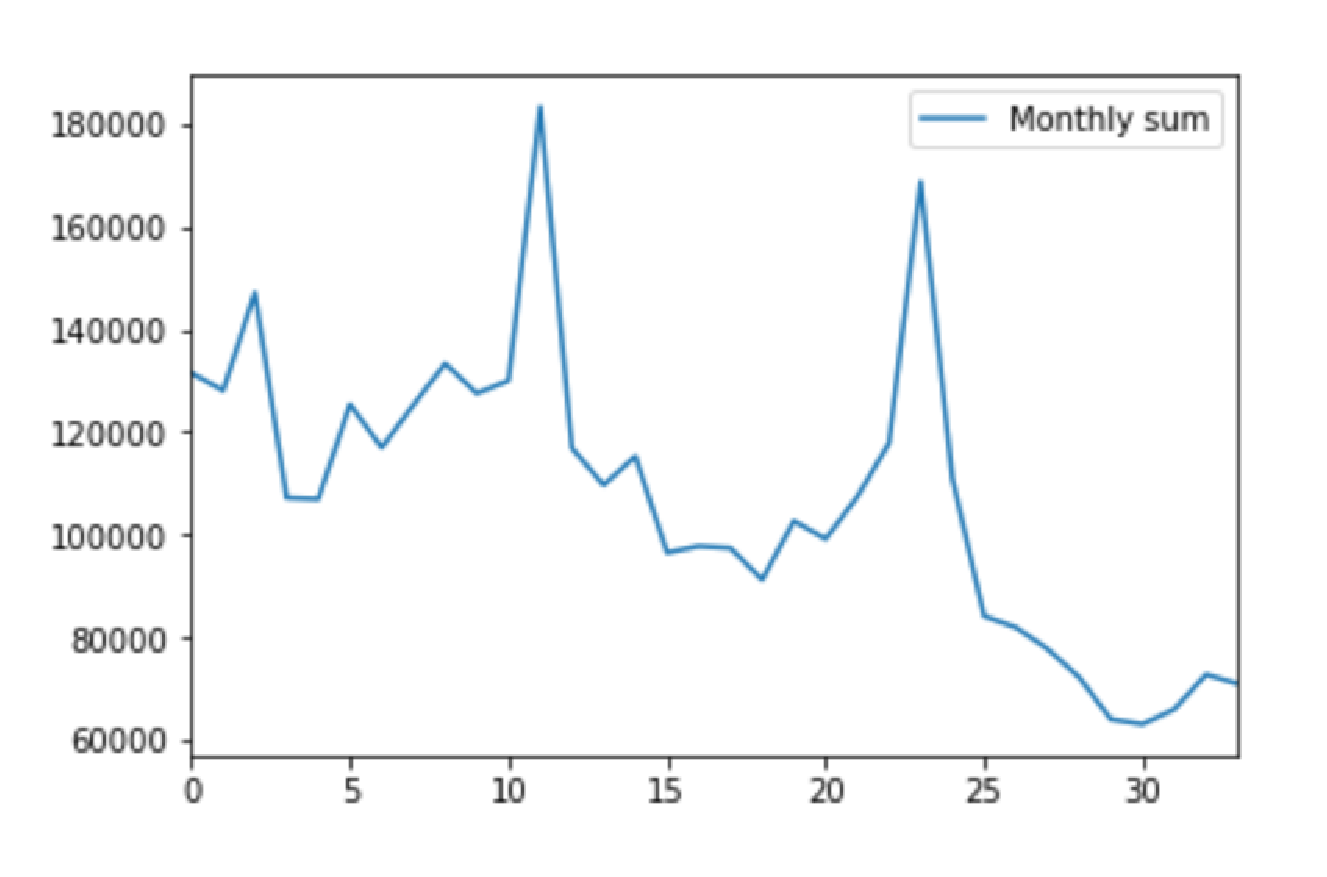
\includegraphics[width=15cm, height=10cm]{figures/sum.eps}
\end{tikzfigure}
    The outliers is obvious by using box plot.
\begin{tikzfigure}%[Overall architecture of \emph{GOAM} algorithm]
	%  \includegraphics[width=0.8\linewidth]{figures//framework.pdf}
	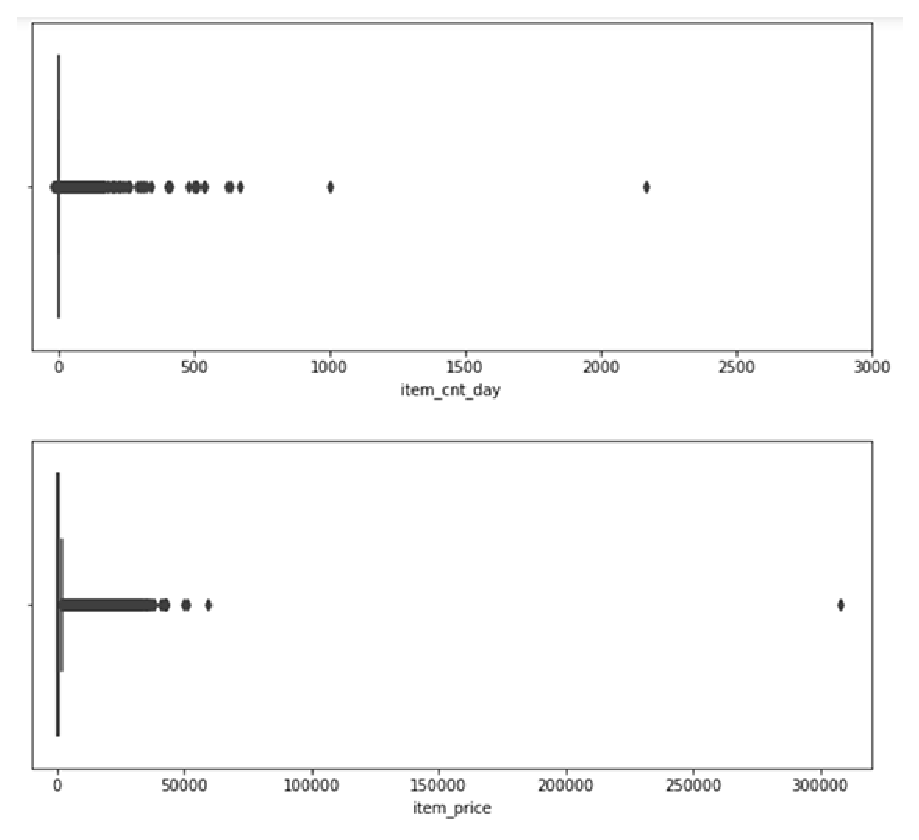
\includegraphics[width=15cm, height=13cm]{figures/outliers.eps}
\end{tikzfigure}
}
%%%%%%%%%% -------------------------------------------------------------------- %%%%%%%%%%


% SECOND column
\column{0.5}
 %Second column with first block's top edge aligned with with previous column's top.

%%%%%%%%%% -------------------------------------------------------------------- %%%%%%%%%%
\block{Feature Selection and Feature Importance}{

\begin{itemize}
	\item Data features which are given
	\begin{description}
		\item
\ shop\_id, item\_id, item\_cnt\_month, shop\_type\_code, shop\_city\_code, year, month, item\_category\_id, item\_type\_code, sub\_type\_code
	\end{description}
	\item Monthly sales features
	\begin{description}
		\item \ average monthly sales of items 
		\item \ average monthly sales of shops 
		\item \ average monthly sales of categories 
		\item \ average monthly sales of types and 
		\item \ subtypes  average monthly sales of shop’s city-item
		\item \ average monthly sales of shop’s type-item
	\end{description}
	\item Historical features
	\begin{description}
		\item \ historical delay:1,2,3,6,12 
	\end{description}
    \item Feature importance
\end{itemize}

\begin{tikzfigure}%[Overall architecture of \emph{GOAM} algorithm]
    \includegraphics[width=30cm, height=15cm]{figures/light.eps}
\end{tikzfigure}
 
}
%%%%%%%%%% -------------------------------------------------------------------- %%%%%%%%%%
% Second column - first block


%%%%%%%%%% -------------------------------------------------------------------- %%%%%%%%%%
\block[titleleft]{Modeling and Result}
{
\begin{itemize}
	\item Model:Lightgbm
	\item Score:0.93740(RMSE)
	\item Rank:3027/8738
\end{itemize}
}
%%%%%%%%%% -------------------------------------------------------------------- %%%%%%%%%%


% Second column - second block
%%%%%%%%%% -------------------------------------------------------------------- %%%%%%%%%%
\block[titlewidthscale=1, bodywidthscale=1]
{Conclusion}
{
 Compare to midterm presentation, RMSE decreased from 1.04885 to 0.93740. The reason mainly is more features and different modeling. In the figure of feature importance and monthly sales, some historical feature play an important role. And lightgbm model's and xgboost model's result have a marginal difference, but processing speed of lightgbm model is faster.

}
%%%%%%%%%% -------------------------------------------------------------------- %%%%%%%%%%


% Bottomblock
%%%%%%%%%% -------------------------------------------------------------------- %%%%%%%%%%

%\note[targetoffsetx=8cm, targetoffsety=-10cm,rotate=0,angle=180,radius=8cm,width=.46\textwidth,innersep=.1cm]{
%Acknowledgement
%}

%\block[titlewidthscale=0.9, bodywidthscale=0.9]
%{Acknowledgement}{
%}
%%%%%%%%%% -------------------------------------------------------------------- %%%%%%%%%%

\end{columns}


%%%%%%%%%% -------------------------------------------------------------------- %%%%%%%%%%
%[titleleft, titleoffsetx=2em, titleoffsety=1em, bodyoffsetx=2em,%
%roundedcorners=10, linewidth=0mm, titlewidthscale=0.7,%
%bodywidthscale=0.9, titlecenter]

%\colorlet{noteframecolor}{blue!20}
\colorlet{notebgcolor}{blue!20}
\colorlet{notefrcolor}{blue!20}
\note[targetoffsetx=-13cm, targetoffsety=-12cm,rotate=0,angle=180,radius=8cm,width=.96\textwidth,innersep=.4cm]
{
\begin{minipage}{0.3\linewidth}
\centering

\includegraphics[width=24cm]{logos/tulip-wordmark.eps}
\end{minipage}
\begin{minipage}{0.7\linewidth}
{ \centering
 Flip00 project report,18/09/2020,changsha,China
}
\end{minipage}
}
%%%%%%%%%% -------------------------------------------------------------------- %%%%%%%%%%


\end{document}

%\endinput
%%
%% End of file `tikzposter-template.tex'.
